\chapter{速度合成、光錐與四維向量}

\section{同一條鐵路軌道上的兩個參考系}

先前推導的洛倫茲變換涉及一種刻意受限的幾何情形：所有相對運動都沿著同一軸向。想像一條長長的鐵路軌道。一組觀測者留在車站，另一組則搭乘沿軌道行駛的列車。橫向方向雖然存在，但要等到稍後納入時才會發揮作用。

每個參考系都是一套操作性座標系。靜止於該參考系的米尺定義空間座標，靜止於該參考系的同步時鐘則定義時間。決定兩者關係的假設是：所有慣性觀測者測得的光速都相同。

大多數計算會使用\(c=1\)。時間可以用秒、距離用光秒來度量，也可以用年和光年來度量。如此一來，速度便是光速的無量綱分數。需要使用一般單位時，可由量綱一致性唯一地補回\(c\)因子；例如，無量綱洛倫茲因子中的\(v^2\)會變為\(v^2/c^2\)。

\subsection{正變換與逆變換}

假設列車內或列車附近某處發生了一次閃光。這是一個事件，不因描述者不同而改變。車站觀測者為它指定座標\((x,t)\)，列車觀測者則指定\((x',t')\)。在\(c=1\)單位制下，
\begin{align}
x'&=\gamma_v(x-vt),&
t'&=\gamma_v(t-vx),
\label{eq:sr2-direct}\\
\gamma_v&=\frac{1}{\sqrt{1-v^2}}.
\end{align}
牛頓會認出位移\(x-vt\)；因子\(\gamma_v\)，以及\(x\)混入\(t'\)的情形，則是相對論帶來的變化。

\begin{figure}[htbp]
\centering
\includegraphics[width=0.90\textwidth]{lecture_02_figure_01.png}
\caption{將車站座標\((x,t)\)與列車座標\((x',t')\)聯繫起來的正向洛倫茲變換。}
\lectureframe{00:07:52}
\end{figure}

由互易性可知，將相對速度的符號反轉即可得到逆變換：
\begin{align}
x&=\gamma_v(x'+vt'),&
t&=\gamma_v(t'+vx').
\label{eq:sr2-inverse}
\end{align}
車站並非絕對靜止；它只是被指定為不帶撇號的參考系，而列車觀察到它以\(-v\)運動。

\begin{figure}[htbp]
\centering
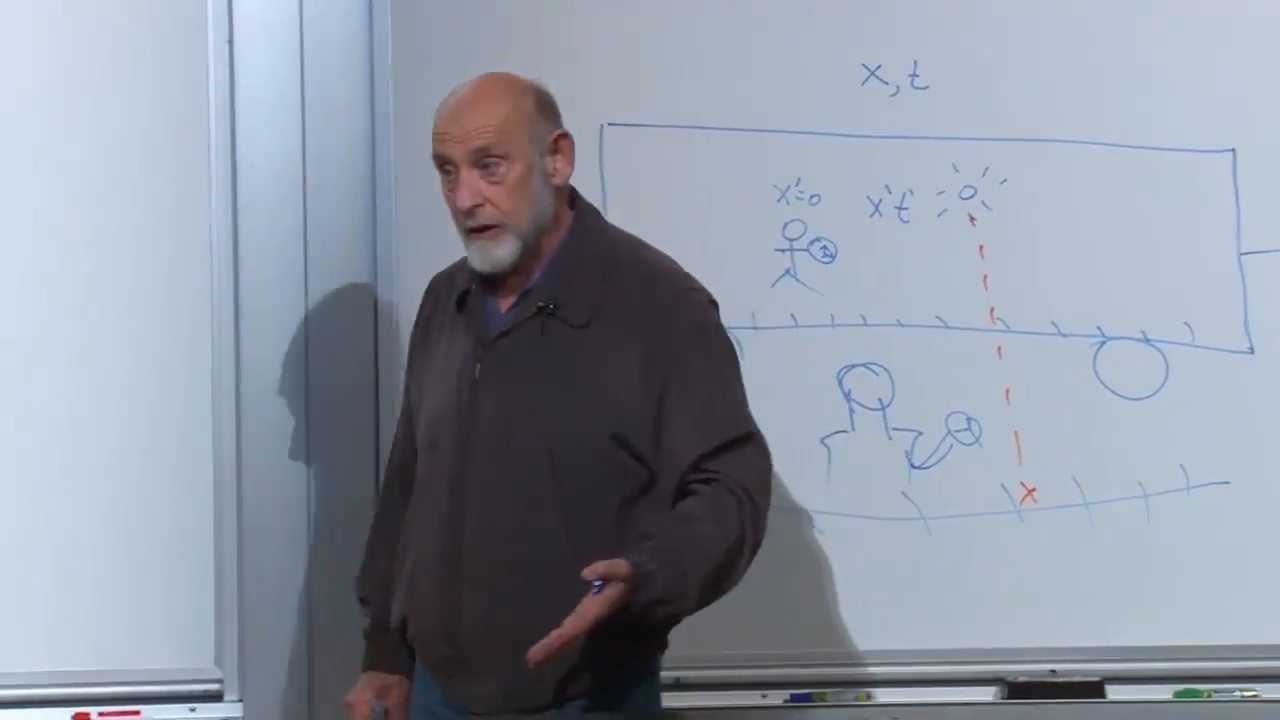
\includegraphics[width=0.90\textwidth]{lecture_02_figure_02.png}
\caption{逆變換具有相同的洛倫茲因子，但相對速度的符號相反。}
\lectureframe{00:09:15}
\end{figure}

對於沿\(x\)方向的推進，橫向座標保持不變：
\begin{equation}
y'=y,
\qquad
z'=z.
\end{equation}

無須研究分母，就能從空間方程讀出相對速率。列車原點由\(x'=0\)定義，因此
\begin{equation}
x'=0
\quad\Longleftrightarrow\quad
x-vt=0
\quad\Longleftrightarrow\quad
x=vt.
\label{eq:sr2-origin-worldline}
\end{equation}
這條世界線中\(t\)的係數，就是列車在車站座標系中的速度。

\section{三個參考系與推進的合成}

在列車裡放一輛小玩具車。列車相對於車站以速度\(v\)運動，而玩具車相對於列車乘客沿著走道以速度\(u\)運動。令玩具車相對於車站的速度為\(w\)。牛頓力學的直覺會預期\(w=u+v\)，但結果仍須由洛倫茲變換來決定。

現在有三個座標系：
\begin{equation}
(x,t),\qquad (x',t'),\qquad (x'',t'').
\end{equation}
第一個屬於車站，第二個屬於列車，第三個屬於玩具車。在列車與玩具車之間，
\begin{align}
x''&=\gamma_u(x'-ut'),&
t''&=\gamma_u(t'-ux'),
\label{eq:sr2-second-boost}\\
\gamma_u&=\frac{1}{\sqrt{1-u^2}}.
\end{align}

\begin{figure}[htbp]
\centering
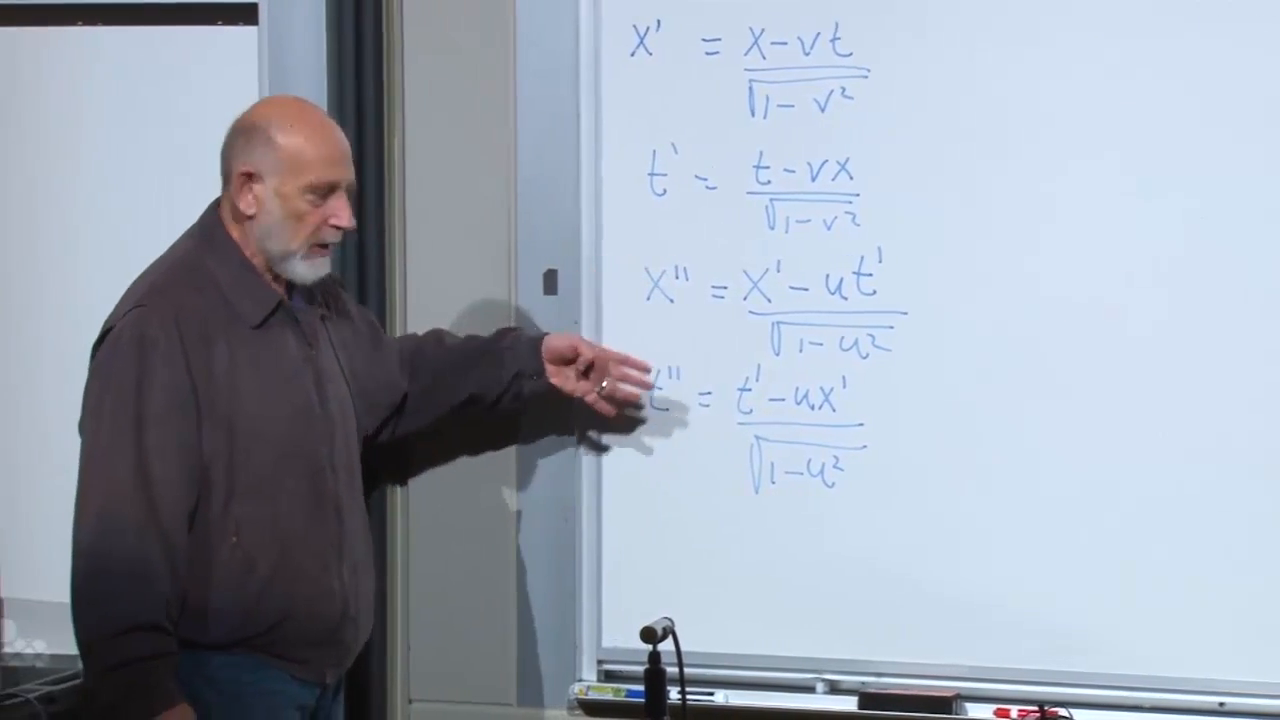
\includegraphics[width=0.90\textwidth]{lecture_02_figure_03.png}
\caption{先寫出車站到列車的正向變換公式，再接著施行第二個洛倫茲變換，將帶撇號的座標變為雙撇號座標。}
\lectureframe{00:14:55}
\end{figure}

\subsection{將一個推進代入另一個}

只用空間方程就足以求出\(w\)。將\eqref{eq:sr2-direct}代入\eqref{eq:sr2-second-boost}的第一個方程：
\begin{align}
x''
&=\gamma_u(x'-ut')\\
&=\gamma_u\gamma_v\left[(x-vt)-u(t-vx)\right]\\
&=\gamma_u\gamma_v\left[(1+uv)x-(u+v)t\right].
\label{eq:sr2-composed-space}
\end{align}
\(uvx\)項中的兩個負號相乘後變成正號；兩個時間項則合併為\(-(u+v)t\)。

\begin{figure}[htbp]
\centering
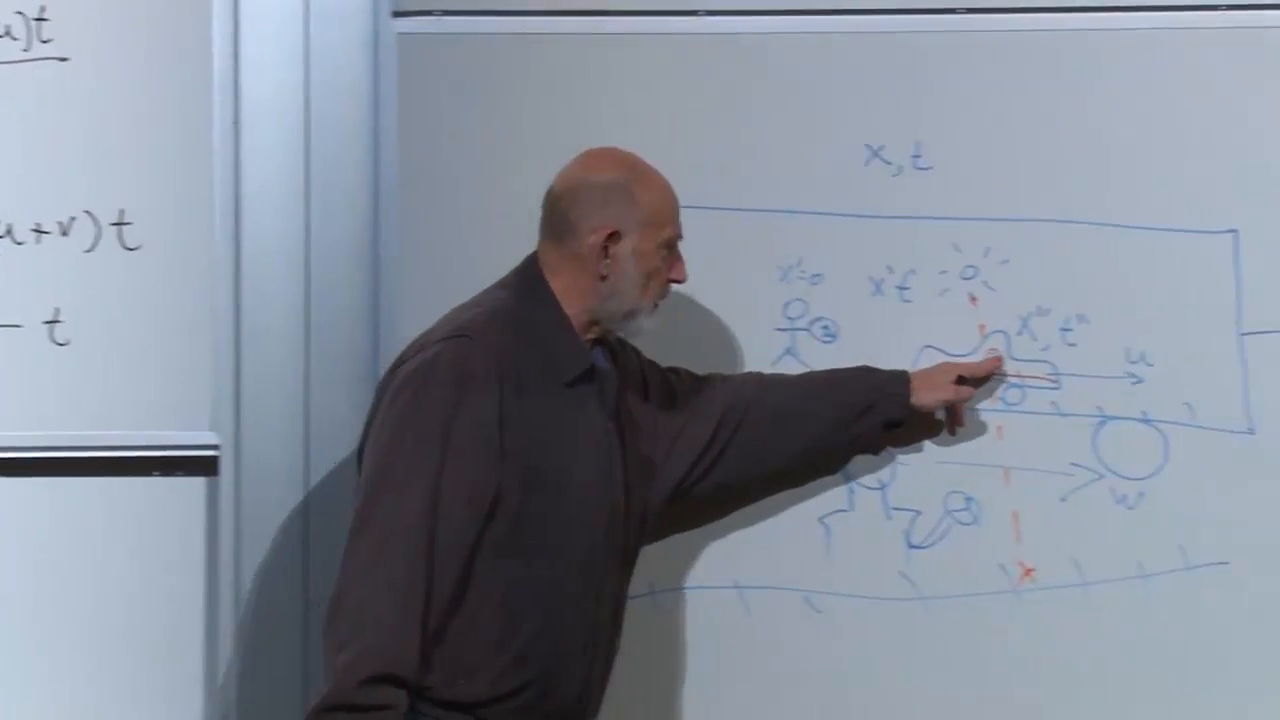
\includegraphics[width=0.91\textwidth]{lecture_02_figure_04.png}
\caption{在合成推進中，收集\(x\)項與\(t\)項之前的巢狀代入。}
\lectureframe{00:16:30}
\end{figure}

和前面一樣，要找出運動原點時，分母無關緊要。玩具車靜止於\(x''=0\)，因此\eqref{eq:sr2-composed-space}中的括號必須為零：
\begin{equation}
(1+uv)x-(u+v)t=0.
\end{equation}
所以，它在車站參考系中的世界線為
\begin{equation}
x=\frac{u+v}{1+uv}\,t,
\end{equation}
其速度則為
\begin{equation}
\boxed{w=\frac{u+v}{1+uv}}.
\label{eq:sr2-velocity-add-c1}
\end{equation}

\begin{figure}[htbp]
\centering
\includegraphics[width=0.91\textwidth]{lecture_02_figure_05.png}
\caption{整理後的分子與世界線\(x=[(u+v)/(1+uv)]t\)揭示了合成速度。}
\lectureframe{00:19:30}
\end{figure}

時間方程的合成也一致。從車站到玩具車的完整變換具有洛倫茲變換的形式
\begin{align}
x''&=\gamma_w(x-wt),&
t''&=\gamma_w(t-wx),
\end{align}
其中
\begin{equation}
\gamma_w=\frac{1}{\sqrt{1-w^2}}.
\end{equation}
事實上，
\begin{equation}
\gamma_w=\gamma_u\gamma_v(1+uv),
\end{equation}
這個關係可由代入\eqref{eq:sr2-velocity-add-c1}並加以化簡得到。因此，兩個共線推進合成後，仍是另一個共線推進。

\subsection{恢復量綱}

\begin{classroomqa}
\audiencequestion{為什麼在一般單位制下，分母\(1+uv\)的量綱不正確？}
\lecturerresponse{它之所以正確，只是因為\(c=1\)使每個速度都成為光速的無量綱分數。在慣用單位制下，乘積必須寫成\(uv/c^2\)，如此才是無量綱的。\lecturetimestamp{00:21:11}}
\end{classroomqa}

具有量綱的速度合成定律為
\begin{equation}
\boxed{
w=\frac{u+v}{1+\dfrac{uv}{c^2}}
}.
\label{eq:sr2-velocity-add}
\end{equation}

\begin{figure}[htbp]
\centering
\includegraphics[width=0.90\textwidth]{lecture_02_figure_06.png}
\caption{量綱一致性要求在乘積\(uv\)下方補上\(c^2\)。}
\lectureframe{00:22:06}
\end{figure}

當\(\lvert u\rvert,\lvert v\rvert\ll c\)時，
\begin{equation}
\frac{uv}{c^2}\ll 1,
\end{equation}
因此
\begin{equation}
w\approx u+v.
\end{equation}
牛頓式速度相加是低速近似，而不是另一條獨立定律。

\subsection{兩種數值情況}

先取
\begin{equation}
u=v=0.01c.
\end{equation}
在\(c=1\)單位制下，
\begin{equation}
w=\frac{0.02}{1.0001}\approx 0.019998.
\end{equation}
光速的百分之一已約為\(3\times10^6\ {\rm m/s}\)，但相對論修正只有萬分之一。結果略小於牛頓力學所預測的\(0.02c\)。

\begin{figure}[htbp]
\centering
\includegraphics[width=0.90\textwidth]{lecture_02_figure_07.png}
\caption{當\(u=v=0.01c\)時，分母與一的差只有\(10^{-4}\)。}
\lectureframe{00:24:23}
\end{figure}

現在取
\begin{equation}
u=v=0.9c.
\end{equation}
牛頓力學會預測\(1.8c\)。相對論則給出
\begin{equation}
\frac{w}{c}
=\frac{0.9+0.9}{1+0.9^2}
=\frac{1.8}{1.81}
\approx 0.9945.
\label{eq:sr2-fast-example}
\end{equation}

\begin{figure}[htbp]
\centering
\includegraphics[width=0.90\textwidth]{lecture_02_figure_08.png}
\caption{兩個\(0.9c\)的速度合成後為\(1.8/1.81\)，仍低於光速。}
\lectureframe{00:25:48}
\end{figure}

連續施行次光速推進，結果不可能超過\(c\)。若\(u<c\)且\(v<c\)，則
\begin{equation}
1-\frac{w}{c}
=
\frac{\left(1-\frac{u}{c}\right)
      \left(1-\frac{v}{c}\right)}
     {1+\frac{uv}{c^2}}
>0.
\end{equation}
每增加一次推進，合成速度都能更接近\(c\)，但永遠不會超過它。在極限情形\(u=c\)下，
\begin{equation}
w=\frac{c+v}{1+v/c}=c.
\end{equation}
光速是速度合成定律的不動點。

\section{座標測量不等於視覺所見}

\begin{classroomqa}
\audiencequestion{如果列車有玻璃車壁，車站觀測者能不能直接看著乘客和玩具車，讀出它們各自的運動？}
\lecturerresponse{洛倫茲變換描述的是使用分布在各處的標尺和同步時鐘所做的座標測量。視覺影像還包含光從不同事件傳到觀測者所需的不同時間。玻璃改變的是所見景象，不是座標關係；若把同一幅影像當成同時取得的資料，就會重新引入相對論所修正的那種同時性假設。\lecturetimestamp{00:27:53}}
\end{classroomqa}

無論當下是否有人看見，一個事件在每個參考系中都有其位置和時間。光學上的視覺效果是合理的研究主題，但需要另外計算光從各個事件傳到眼睛的過程。變換定律本身具有普遍性，與列車是否有車壁無關。

\section{三維空間中的固有間隔}

回到兩個事件：其中一個起初位於原點，另一個位於\((x,t)\)。在一維空間中，
\begin{equation}
\tau^2=t^2-x^2
\label{eq:sr2-interval-1d}
\end{equation}
在\(c=1\)單位制下，所有慣性參考系都同意：
\begin{equation}
\tau^2
=t^2-x^2
=t'^2-x'^2
=t''^2-x''^2.
\end{equation}
座標會改變，固有間隔則不變。

若兩事件之間是類時分隔，便可以有一個時鐘在兩事件之間移動。如果它在第一個事件發生時讀數為正午，那麼到第二個事件發生時，時鐘所記錄的經過時間就是固有時間\(\tau\)。無論使用哪個座標參考系計算間隔，這個敘述都成立。

\begin{figure}[htbp]
\centering
\includegraphics[width=0.90\textwidth]{lecture_02_figure_09.png}
\caption{在恢復橫向方向之前，先回顧固有時間的不變關係\(\tau^2=t^2-x^2\)。}
\lectureframe{00:30:18}
\end{figure}

\subsection{以空間旋轉恢復橫向方向}

先考慮空間座標軸的普通旋轉，再回到推進。一個不在\(x\)軸上的點，其空間距離平方為
\begin{equation}
r^2=x^2+y^2+z^2,
\end{equation}
根據一般的畢氏定理，這個距離在旋轉下保持不變。因此，\(3+1\)時空間隔為
\begin{equation}
\boxed{
\tau^2=t^2-x^2-y^2-z^2
}.
\label{eq:sr2-interval-3d}
\end{equation}
恢復\(c\)後，
\begin{equation}
c^2\tau^2
=c^2t^2-x^2-y^2-z^2.
\end{equation}

\begin{figure}[htbp]
\centering
\includegraphics[width=0.90\textwidth]{lecture_02_figure_10.png}
\caption{利用畢氏定理計算的空間距離，將不變量從\(t^2-x^2\)推廣為\(t^2-x^2-y^2-z^2\)。}
\lectureframe{00:34:23}
\end{figure}

空間旋轉與洛倫茲推進的任意組合都會保持\eqref{eq:sr2-interval-3d}不變。一般座標軸對各分量的值未必一致，但都同意歐幾里得距離；慣性時空參考系對空間和時間分量的值未必一致，但都同意這個平方差。這項不變性是狹義相對論的核心幾何事實。

\begin{classroomqa}
\audiencequestion{如果乘客把玩具車換成一束向前照射的手電筒光束，列車觀測者和車站觀測者測得的光速會相同嗎？}
\lecturerresponse{在\eqref{eq:sr2-velocity-add}中令\(u=c\)。於是\(w=(c+v)/(1+v/c)=c\)。在\(c=1\)單位制下，這個比值就是\((1+v)/(1+v)=1\)。兩個參考系測得的速度相同，完全符合要求。\lecturetimestamp{00:35:53}}
\end{classroomqa}

因此，先前對玻璃車壁的疑慮並不表示光速不變原理失效，而是混淆了座標測量與延遲的視覺影像；歸根究柢，這是對同時性的混淆。

\section{零光線與光錐}

在一維空間中，向右與向左行進的光線滿足
\begin{equation}
x=\pm t.
\end{equation}
它們的時空間隔為零：
\begin{equation}
t^2-x^2=0.
\end{equation}
不同於歐幾里得距離，時空間隔為零並不表示事件必須重合，而是表示光訊號能夠連接這些事件。

納入所有空間方向後，光線滿足
\begin{equation}
t^2-x^2-y^2-z^2=0,
\label{eq:sr2-null}
\end{equation}
或者
\begin{equation}
r=t
\end{equation}
在\(c=1\)單位制下，這表示光沿未來方向傳播。

\begin{figure}[htbp]
\centering
\includegraphics[width=0.90\textwidth]{lecture_02_figure_11.png}
\caption{任意空間方向的光都沿著零軌跡傳播，並滿足\(t^2-(x^2+y^2+z^2)=0\)。}
\lectureframe{00:39:28}
\end{figure}

在\(1+1\)維時空中，零集合是兩條\(45^\circ\)直線。加入兩個空間維度和時間維度後，它便成為一個圓錐；三個空間維度無法在黑板上完整呈現，但定義方程並未改變。

未來光錐由從原點發出的光能到達的事件所構成。過去光錐則由光能從該處到達原點的事件所構成。兩者互為時間反轉。

\begin{figure}[htbp]
\centering
\includegraphics[width=0.90\textwidth]{lecture_02_figure_12.png}
\caption{在較高維度的時空圖中，\(45^\circ\)零光線向外展開，形成未來光錐與過去光錐。}
\lectureframe{00:40:47}
\end{figure}

\begin{classroomqa}
\audiencequestion{牛頓力學中的伽利略變換，對應的不變量是什麼？}
\lecturerresponse{時間間隔本身。牛頓力學中的觀測者都同意\(\Delta t\)，即使他們對空間位移的測量不同。相對論放棄了絕對時間，改以不變的時空間隔取而代之。\lecturetimestamp{00:41:53}}
\end{classroomqa}

\section{從空間向量到四維向量}

這裡所說的向量是幾何向量，而不是量子態向量。普通空間中兩點之間的位移具有大小和方向。將向量的尾端平移至原點，不會改變向量；它的三個分量可記為
\begin{equation}
x^i=(x^1,x^2,x^3)=(x,y,z),
\qquad i=1,2,3.
\end{equation}
拉丁指標\(i\)只涵蓋空間方向。

事件還需要一個額外分量，也就是時間。因此，時空位置寫作
\begin{equation}
x^\mu=(x^0,x^1,x^2,x^3)=(t,x,y,z),
\qquad \mu=0,1,2,3.
\label{eq:sr2-four-position}
\end{equation}
依照歷史慣例，時間列為第零分量，而不是第四分量：
\begin{equation}
x^0=t,\qquad x^1=x,\qquad x^2=y,\qquad x^3=z.
\end{equation}
希臘指標，例如\(\mu\)，涵蓋時空分量；拉丁指標，例如\(i\)，則涵蓋空間分量。

\begin{figure}[htbp]
\centering
\includegraphics[width=0.90\textwidth]{lecture_02_figure_13.png}
\caption{空間分量\(x^i\)擴展為四分量的時空位置\(x^\mu=(x^0,x^1,x^2,x^3)\)。}
\lectureframe{00:46:05}
\end{figure}

不變量變為
\begin{equation}
\tau^2
=(x^0)^2-(x^1)^2-(x^2)^2-(x^3)^2.
\end{equation}
光是引入這套記號，並不會帶來新的物理內容。它的價值在於洛倫茲變換會線性地作用於全部四個分量，就像旋轉會線性地作用於空間向量一樣。

\begin{classroomqa}
\audiencequestion{既然變換是線性的，能不能用作用於列向量的矩陣來表示？}
\lecturerresponse{可以。對於沿\(x\)方向的推進，非平凡的矩陣區塊\(\gamma_v\begin{pmatrix}1&-v\\-v&1\end{pmatrix}\)作用於\((t,x)^{\mathsf T}\)；而\(y\)和\(z\)保持不變。矩陣記法很適合用來組合和整理洛倫茲變換。\lecturetimestamp{00:48:14}}
\end{classroomqa}

明確寫出來就是
\begin{equation}
\begin{pmatrix}
t'\\x'\\y'\\z'
\end{pmatrix}
=
\begin{pmatrix}
\gamma_v&-\gamma_v v&0&0\\
-\gamma_v v&\gamma_v&0&0\\
0&0&1&0\\
0&0&0&1
\end{pmatrix}
\begin{pmatrix}
t\\x\\y\\z
\end{pmatrix}.
\label{eq:sr2-boost-matrix}
\end{equation}

\section{位移與四維速度}

從一個事件的位置沿著粒子的世界線前進一小段。四維位移為
\begin{equation}
\Delta x^\mu
=(\Delta t,\Delta x,\Delta y,\Delta z).
\end{equation}
說位移很小時，就是要進入微積分的描述：\(\Delta x^\mu\)將變為\(dx^\mu\)。目前先使用有限的表示法，幾何關係會更加清楚。

類時世界線上的固有時間增量滿足
\begin{equation}
(\Delta\tau)^2
=(\Delta t)^2-(\Delta x)^2-(\Delta y)^2-(\Delta z)^2.
\label{eq:sr2-proper-increment}
\end{equation}
普通速度是用座標時間除空間位移，具有三個分量。四維速度則是用不變的固有時間除四維位移：
\begin{equation}
u^\mu
=\frac{\Delta x^\mu}{\Delta\tau}
\quad\longrightarrow\quad
\boxed{
u^\mu=\frac{dx^\mu}{d\tau}
}.
\label{eq:sr2-four-velocity}
\end{equation}

\begin{figure}[htbp]
\centering
\includegraphics[width=0.90\textwidth]{lecture_02_figure_14.png}
\caption{一段世界線定義了\(\Delta x^\mu\)、其不變量\(\Delta\tau\)，以及四維速度\(u^\mu=\Delta x^\mu/\Delta\tau\)。}
\lectureframe{00:52:42}
\end{figure}

這個量具有四個分量，並依四維向量的方式變換。它與普通三維速度的關係，就是接下來要探討的問題；此處刻意先不回答。釐清這個關係，將引向相對論動量、能量、加速度，最終則是\(F=ma\)的相對論推廣。
